\chapter{Proposed approach}
\label{chapter:proposedApproach}


\section{Feature specification}
\label{section:featureSpecification}

Now that we have analyzed the technical requirements and identified some of the challenges that could be encountered, we can continue with defining the solution for the described problem. Our approach would involve designing and developing a web application, keeping in mind its advantages over desktop applications, which we described in the previous section. The app would include two major parts: a web service developed in Java using the Spring Boot Framework and a client app built using the ReactJS Framework. The web sevice will define a REST API which will be used for communication between the client and the server. It will also handle the business logic and manage the persistence of data, which will be achieved by using a MySQL database. The client app will be the one that will run in the user's browser. As REST is stateless by definition, the client app will have to manage the session state. This will be achieved with the help of Redux - a predictable state container for JavaScript apps.

One important thing to keep in mind is that the application will be used for managing real documents of a public institution, which could potentially involve sensitive data. To secure our app, we will use features offered by Spring Security to enable JSON Web Token Authentication and manage access control.



\section{Technologies used}
\label{section:technologiesUsed}

In the following subsections of this chapter we will describe each of the chosen technologies in detail, with a strong focus on features that were decisive in choosing it over alternative technologies from the same branch.


\subsection{The Spring Framework}
\label{subsection:theSpringFramework}

The Spring Framework is an application framework for the Java platform which offers a wide range of features for modern Java-based applications. According to a survey from 2018, Spring is the most popular Web Framework worldwide in the JVM ecosystem (See Figure \ref{javaWebFrameworksTrendsImg}). It provides a large set of functionality and tools, making it suitable for a big variety of applications. In addition, its flexibility and focus on ease of use allow developers to focus on the application business logic rather than configurations and boilerplate code, thus increasing velocity, productivity and development speed.

\begin{figure}[H]
    \centering
    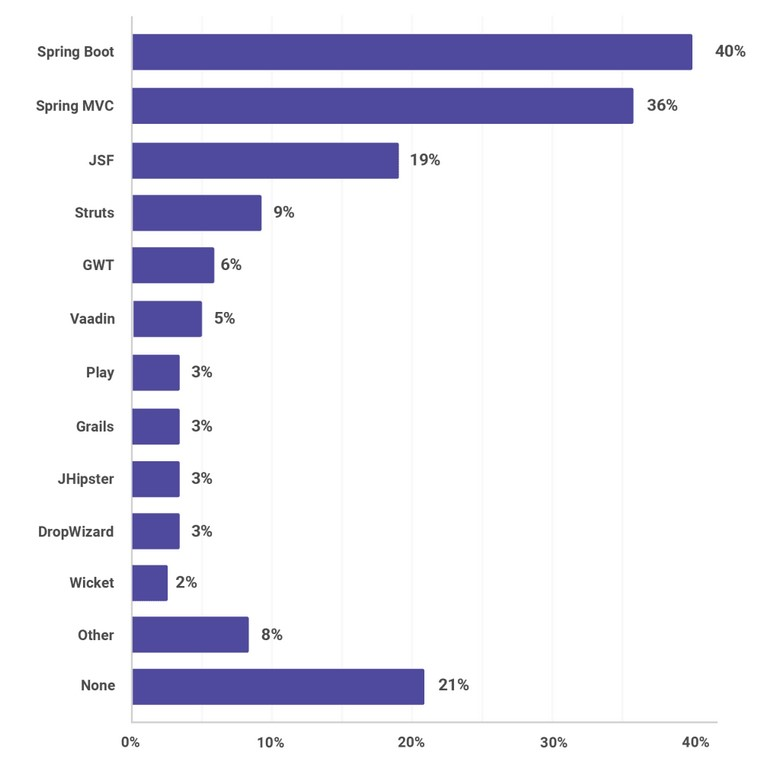
\includegraphics[width=4in]{images/javaWebFrameworksTrends}
    \caption{The most popular Java Web Frameworks according to the JVM Ecosystem report 2018 \cite{jvmEcosystemReport}}
    \label{javaWebFrameworksTrendsImg}
\end{figure}

One of the most important features offered by Spring is \textit{Inversion of Control} (IoC), achieved by \textit{Dependency Injection} (DI). According to this principle, objects are not responsible for creating their dependencies. Instead, they should be "injected" into the object through arguments passed to the constructor, setter methods or factory methods. In contrast to the classical way where each object is locating and instantiating all of its dependencies, the DI approach has several advantages. The most important one is achiving loose coupling, making it easier to interchange distinct implementations and maintain program modularity.

To achieve this, the Spring Framework uses an \textit{IoC container}. It is responsible for the instantiation, configuration and managing of the \textit{beans} - objects that will be used by the application (See Figure \ref{springIocContainer}). In order to know how each bean should be created and which dependencies injected, the IoC container needs additional configuration information. This is provided as metadata in form of XML, Java Configuration classes or Java annotations. In our project, we are going to use Java annotations as it is the most easy and straightforward way to configure beans.

\begin{figure}[H]
    \centering
    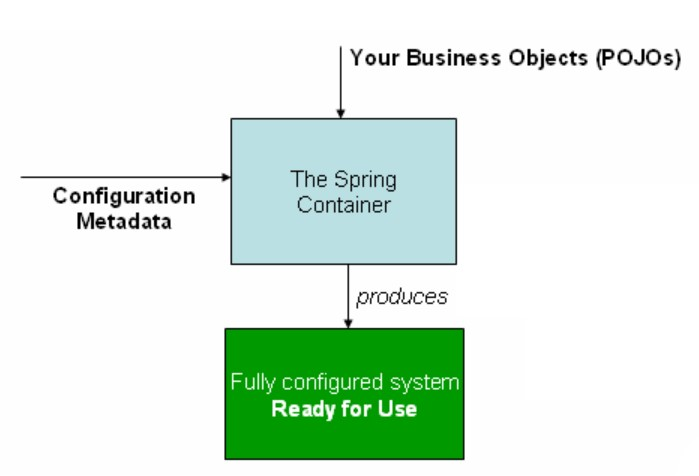
\includegraphics[width=4in]{images/springIocContainer}
    \caption{The Spring IoC Container \cite{springDocs}}
    \label{springIocContainer}
\end{figure}

Another advantage of Spring is that it uses well-known design patterns which are implemented under the hood:

\begin{itemize}
    \item All beans created by Spring are by default \textbf{Singletons}. This means that the IoC container creates only one instance for a bean and caches it so that it could then be used in multiple different places.
    \item Spring uses the \textbf{Factory Method Pattern} for bean creation. The \code{BeanFactory} class defines a list of \code{getBean()} methods, all of each are factory methods that could be used to create a bean with the desired configuration. This functionality is extended by the \code{ApplicationContext} class, which adds the posibility of creating beans using external configurations like XML files or Java annotations.
    \item Spring uses the \textbf{Proxy Pattern} to control access to its beans. One tipical example where this is necessary is when using transactions. If we annotate a method as \code{@Transactional}, Spring guarantees its atomic execution and transactional consistency (hence the name). This is only possbile by intercepting the call through a proxy object that wraps our bean and would control the method execution.
    \item Spring uses the \textbf{Template Method Pattern} to minimize the amount of boilerplate code that is repeated again and again throughout projects. The \code{JdbcTemplate} class is a perfect example, providing an easy and intuitive way to execute database queries using predefined templates.
\end{itemize}


\subsection{Spring Boot}
\label{subsection:springBoot}

The Spring Framework provides a wide range of features for building enterprise and web applications, which makes it suitable for almost any type of use case. However, with the increasing amount of Spring features embedded into an application, the complexity of developing it also increases. Configurations grow in size and get difficult to maintain.

Spring Boot was designed to solve exactly this problem. The module, while maintaining all of the power of its parent, significantly reduces the amount of configurations the developer has to make. It eliminates the need to write those parts of the code that always tend to be the same across multiple projects, like configuring a data source or a transaction manager. It also tends to simplify the deployment process, offering an embedded server which is ready to run as an alternative to manually setting up a deployment server.

As for managing external dependencies, Spring Boot comes with the new concept of \textit{starters} - dependency descriptors which bundle together multiple dependencies that are usually used together for achieving a task. Our project is a good example that illustrates the usage of this feature. Developing a web service requires multiple external modules: we would use features from different Spring modules, but then we would also need libraries that would take care of parameter validaton, JSON conversions and server embedding. Spring Boot assumes this set of libraries would be required in most web services, and wraps them all in a \code{spring-boot-starter-web} dependency. By including this dependency in our project it transitively imports all dependencies it contains, saving us the effort of including each one manually.

All of these features result in an effortless development of web applications, which has made Spring Boot a widely popular choice for developing RESTful web services.


\subsection{Spring Security and JWT}
\label{subsection:springSecurityAndJWT}

The Spring Security framework provides \textit{authentication} and \textit{authorization} support for Spring-based applications. We will try to explain this concepts on the example of our application. One of its main features is storing documents in an online archive. Authentication will provide users access to the document archive, so that they can see the entire list of registered documents and basic details like the person who submitted them or the registration date. On the other hand, authorization will give a user permission to perform more specific actions, like download the file content associated with the document or mark it as resolved.

Traditionally, Spring Security operates by creating a session and storing cookies on the client. However, this contradicts the principles of REST architecture.

To avoid this, we are going to use JSON Web Tokens which handle authentication in a stateless way and can be easily integrated with Spring Security. As stated in \cite{buildingRESTfulWebServicesWithSpring}, a JWT is just a string consisting of three encoded parts which are separated by a dot:

\begin{itemize}
    \item The \textbf{header} is used to indicate the hashing algorithm used to sign the token. In our application we use the \textit{HS512} - a Hash-based Message Authentication Code algorithm which uses the SHA-512 cryptographic hash function and a secret cryptographic key to generate the code.
    \item The \textbf{payload} is used to store the user's \textit{claims} - information about the user like authorization data, roles and permissions.
    \item The \textbf{signature} is the final section of the token used for additional verifications.
\end{itemize}

The way JWT secures the application is simple and intuitive (\ref{jwtFlow}). When the user enters his or her credentials in the login form, they are sent to the server for verification. If the provided credentials are correct, the server queries the database for information about the user, generates a JWT and stores the user information in it. The server has to also specify an expiration time for the token. After being signed and hashed, the JWT is sent to the client as a response to the authentication request. As the server is stateless, it is the clients responsibility to store the token until it expires.

Afterwards, every request from the client to the server has to contain the JWT token specified in an Authorization header. The server will extract the token, validate the signature and get the user data from the JWT payload. Based on that data, the server will decide if the user is or is not authorized to perform the desired request.

\begin{figure}[H]
    \centering
    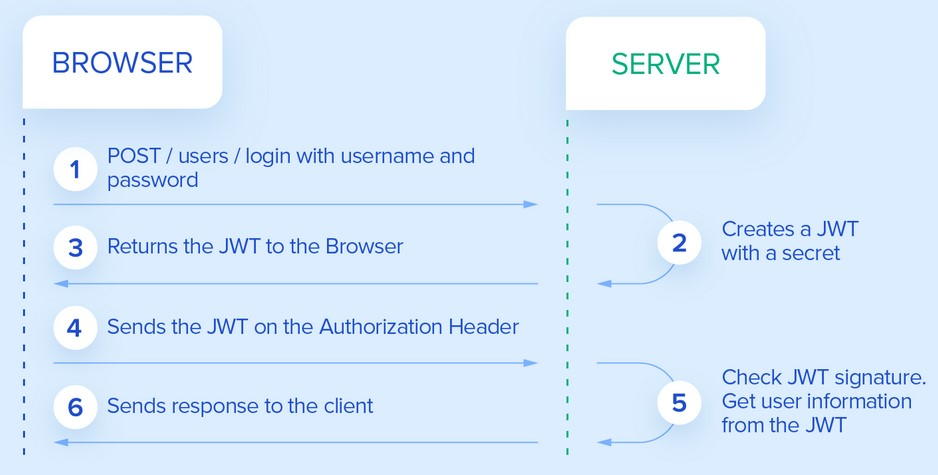
\includegraphics[width=5in]{images/jwtFlow}
    \caption{Creation and usage of Json Web Tokens \cite{jwtFlow}}
    \label{jwtFlow}
\end{figure}


\subsection{MySQL Database}
\label{section:mysqlDatabase}

An important decision we had to make was whether to choose a \textit{relational} or a \textit{non-relational} database for persisting our data. Relational databases have been successfully used in enterprise applications for decades, however the NoSQL movement of the recent years has questioned whether the relational model is the best approach in all situations. Indeed, relational databases weren't designed to be used in an Object Oriented context. There are numerous techniques of mapping domain objects into database tables and columns. It is especially cumbersome when concepts like inheritance or user-defined data types are involved. The normalization of the obtained database model usually tends to split the information about an entity across multiple tables. We then need to make use of the foreign keys and perform joins to reconstruct our entity, which are costly operations. This is the main reason why, in the Big Data Era, non-relational databases are prefered for storing huge amounts of data. A NoSQL database will store information as JSON documents instead of rows spread across multiple tables, which will provide a considerable advantage in scalability and performance.

The drawback is that NoSQL databases don't treat operations as transactions. This makes the non-relational model a less fitted choice if you have operations that depend on each other and all of them must either execute successfully or not at all (See \cite{conciseGuideToDatabases}). In our application, ensuring consistency of the persisted data is key. We want to enforce data integrity by maintaining the \textit{ACID} principles (Atomicity, Consistency, Isolation, Durability). That is the reason why a relational database seems the most fitted choice for our application.

From the vast amount of relational database technologies available, we chose to use \textbf{MySQL}, which is an open-source relational database management system. To compensate for the speed - the field where non-relational databases are performing better than relational ones, we will research techniques to improve MySQL query performance described in \cite{highPerformanceMySQL}. One basic technique for increasing the speed of operations is using \textit{indexes} - data structures that boost data management efficiency and become increasingly important as the size of managed data grows. There are also different types of indexes to consider. Tree-based indexes are more suited for fields which will be accessed with range queries or for sorting the query results. Thus it would make sense to create a \textit{B-Tree} index on fields based on which we will sort documents in our application - like, for instance, the document registry number. Hash-based indexes, on the other hand, perform better for direct access. In our database, a \textit{Hash} index would be useful for the email column of the user table, as the user retrieval at login time will be performed based on email instead of the id.


\subsection{Spring JDBC}
\label{section:springJdbc}

Next thing to consder is how the web service is going to connect to the database. Spring boot offers support for multiple Object Relational Mapping (ORM) frameworks, such as Hibernate and JPA. This are sometimes preferred because the developer doesn't have to think about how the data is stored. The mapping between the object-oriented world and the database is handled entirely by the framework. However, this might not always result in fully optimized queries. This is why, for our application, we chose the \textbf{Spring JBDC} Database Access. With this approach, the Spring Framework is still fully responsile for managing low-level details like opening and closing the connection, preparing and executing the statement and handling transactions. What we get instead is having full control over SQL statements and query parameters. The \code{NamedParameterJdbcTemplate} also offers the possibility to provide names for each parameter instead of the classical unintuitive placeholders (\code{?}), which results in a more readable and less error-prone code.


\subsection{ReactJS Framework}
\label{section:reactJSFramework}

With the rise of the popularity of web applications, front-end technologies have also become a rather popular topic. In constrast to using plain old HTML and JavaScript, modern UI frameworks strive to offer solutions for achieving a responsive and interactive user interface with minimum effort.

\begin{figure}[H]
    \centering
    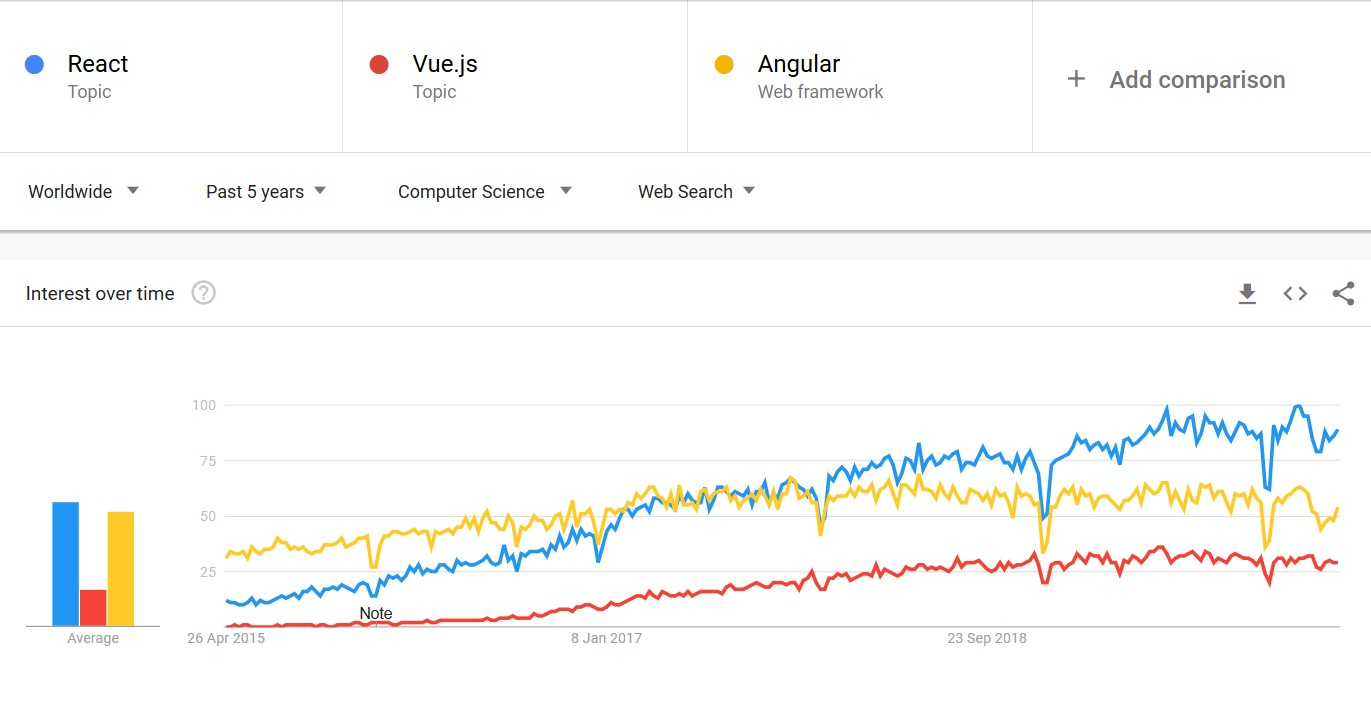
\includegraphics[width=6.5in]{images/jsWebFrameworksTrends}
    \caption{Popularity of JavaScript front-end frameworks in the last 5 years according to Google Trends}
    \label{jsWebFrameworksTrends}
\end{figure}

\textbf{React}, \textbf{Vue.js} and \textbf{Angular} are 3 popular JavaScript frameworks that have been constantly present in front-end technologies tops in the last years. According to Google Trends (Figure \ref{jsWebFrameworksTrends}), the popularity of Angular has been falling since 2015, while the interest for both React and Vue has been rising. However, React has a greater popularity, since Vue is a younger technology with a smaller community.

All of them tend to offer similar features like component-based architecture that results in reusable components, easy syntax and high performance. However, for our application we chose to use React as our UI framework. In comparison to Angular, it is more lightweight and thus suitable for systems that aren't too complex. As for Vue.js, it is a progressive fast-changing framework which is steadily gaining popularity, but React has the advantage of being on the market for a longer time, which guarantees reliability of the resulting software.


\subsection{Redux}
\label{section:redux}

According to the official documentation, Redux is \textit{"a predictable state container for JavaScript Apps"}. To put this in simple words, it is a library for managing application state, that can be used standalone or in connection with libraries like React. As described in \cite{tamingTheStateInReact}, state is an overall broad concept that could refer to anything that is present and can be modified in the browser. Entity state is data retrieved from the backend - like the list of all documents or the object describing the user that is currently logged in to the application. On the other hand, view state is not stored in the backend and is only related to the UI, like the flag that tells if a dropdown is open or not.

When speaking about state management, we mean initializing, modifying and deleting state. For very small applications, this could be easily handled only by using React's local state. However, as the size and complexity of the application grows, so does the effort needed to manage its state. To make things easier, we used Redux, which handles state management in a predictable and elegant way using only 3 main building parts (See Figure \ref{reduxFlow}):

\begin{itemize}
    \item The \textbf{store} is the most important part, which holds the entire application state as a global object. It is a singleton, meaning that there is only one Redux store per application.
    \item \textbf{Actions} are events that send data from the application to the store. To execute an action in Redux is called to \textit{dispatch}, and it should be done when you want to change the state. Dispatching an action requires providing an \textit{action type} and an additional \textit{payload} - information being sent to the store. Once an action is dispatched, it will pass through all reducers.
    \item \textbf{Reducers} are pure functions that are responsible for updating the state. They take as input the current application state and a dispatched action, and, based on the action type and payload, return the next state. It is worth noting that reducers return a new state object without mutating the current state, which always results in a predictable outcome.
\end{itemize}

\begin{figure}[H]
    \centering
    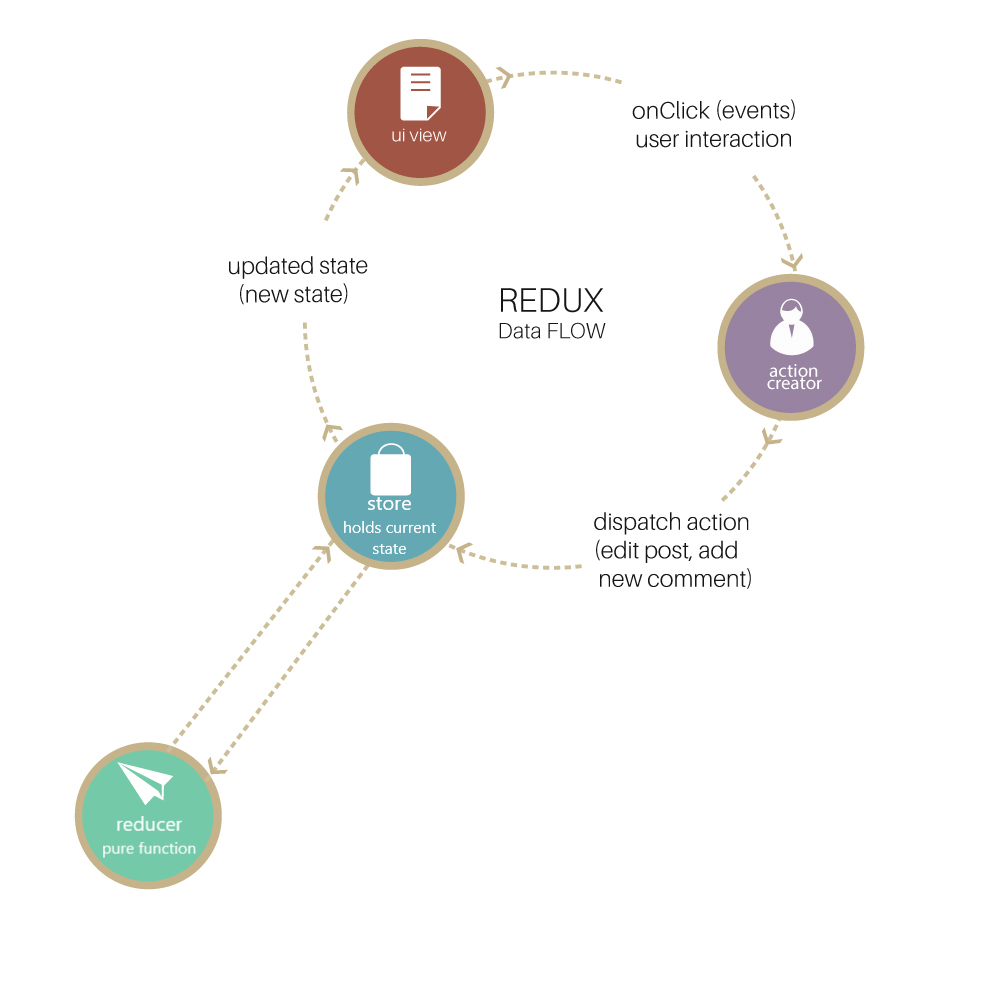
\includegraphics[width=5in]{images/reduxDataFlow}
    \caption{Redux Data Flow \cite{reduxFlow}}
    \label{reduxFlow}
\end{figure}



